% Options for packages loaded elsewhere
\PassOptionsToPackage{unicode}{hyperref}
\PassOptionsToPackage{hyphens}{url}
\documentclass[
  10pt,
  a4paper,
  twocolumn]{article}
\usepackage{xcolor}
\usepackage[top=1.8cm,bottom=1.8cm,left=1.5cm,right=1.5cm]{geometry}
\usepackage{amsmath,amssymb}
\setcounter{secnumdepth}{-\maxdimen} % remove section numbering
\usepackage{iftex}
\ifPDFTeX
  \usepackage[T1]{fontenc}
  \usepackage[utf8]{inputenc}
  \usepackage{textcomp} % provide euro and other symbols
\else % if luatex or xetex
  \usepackage{unicode-math} % this also loads fontspec
  \defaultfontfeatures{Scale=MatchLowercase}
  \defaultfontfeatures[\rmfamily]{Ligatures=TeX,Scale=1}
\fi
\usepackage{lmodern}
\ifPDFTeX\else
  % xetex/luatex font selection
  \setmainfont[]{Times New Roman}
  \setsansfont[]{Arial}
  \setmonofont[]{Menlo}
\fi
% Use upquote if available, for straight quotes in verbatim environments
\IfFileExists{upquote.sty}{\usepackage{upquote}}{}
\IfFileExists{microtype.sty}{% use microtype if available
  \usepackage[]{microtype}
  \UseMicrotypeSet[protrusion]{basicmath} % disable protrusion for tt fonts
}{}
\makeatletter
\@ifundefined{KOMAClassName}{% if non-KOMA class
  \IfFileExists{parskip.sty}{%
    \usepackage{parskip}
  }{% else
    \setlength{\parindent}{0pt}
    \setlength{\parskip}{6pt plus 2pt minus 1pt}}
}{% if KOMA class
  \KOMAoptions{parskip=half}}
\makeatother
\usepackage{longtable,booktabs,array}
\newcounter{none} % for unnumbered tables
\usepackage{calc} % for calculating minipage widths
% Correct order of tables after \paragraph or \subparagraph
\usepackage{etoolbox}
\makeatletter
\patchcmd\longtable{\par}{\if@noskipsec\mbox{}\fi\par}{}{}
\makeatother
% Allow footnotes in longtable head/foot
\IfFileExists{footnotehyper.sty}{\usepackage{footnotehyper}}{\usepackage{footnote}}
\makesavenoteenv{longtable}
\setlength{\emergencystretch}{3em} % prevent overfull lines
\providecommand{\tightlist}{%
  \setlength{\itemsep}{0pt}\setlength{\parskip}{0pt}}
% Publication layout additions for the CystoDS Vietnamese manuscript.
\PassOptionsToPackage{table,xcdraw}{xcolor}
\usepackage{pdflscape}
\usepackage[section]{placeins}
\usepackage{caption}
\usepackage{fancyhdr}
\usepackage{titlesec}
\usepackage{enumitem}
\usepackage{ragged2e}
\usepackage{seqsplit}
\usepackage{booktabs}
\usepackage{changepage}
\usepackage{graphicx}
\usepackage{microtype}
\usepackage{tabularx}
\usepackage{adjustbox}

\definecolor{CystoBlue}{HTML}{1F4E79}
\definecolor{CystoTeal}{HTML}{2A7F62}
\definecolor{CystoGray}{HTML}{4A5568}
\definecolor{CystoDark}{HTML}{1A202C}
\definecolor{CystoLightBg}{HTML}{F7FAFC}

\graphicspath{{../../Docs/}{Docs/}{paper_assets/}}

\captionsetup{font=small,labelfont={bf,color=CystoBlue}}
\captionsetup[table]{position=top,skip=3pt}
\captionsetup[figure]{position=bottom,skip=4pt}

\renewcommand{\figurename}{Hình}
\renewcommand{\tablename}{Bảng}
\renewcommand{\contentsname}{Mục lục}

\titleformat{\section}
  {\large\bfseries\color{CystoBlue}}
  {\thesection.}{0.4em}{}
\titleformat{\subsection}
  {\normalsize\bfseries\color{CystoTeal}}
  {\thesubsection.}{0.4em}{}
\titleformat{\subsubsection}
  {\small\bfseries\color{CystoDark}}
  {\thesubsubsection.}{0.4em}{}

\titlespacing*{\section}{0pt}{1.5ex plus 0.4ex minus 0.2ex}{0.6ex}
\titlespacing*{\subsection}{0pt}{1.2ex plus 0.3ex minus 0.2ex}{0.4ex}
\titlespacing*{\subsubsection}{0pt}{1.0ex plus 0.2ex minus 0.2ex}{0.3ex}

\setlength{\parindent}{1.0em}
\setlength{\parskip}{0.22em plus 0.05em minus 0.05em}
\setlength{\emergencystretch}{3em}
\setlength{\columnsep}{0.65cm}
\setlength{\tabcolsep}{4pt}
\renewcommand{\arraystretch}{1.15}
\setlist{nosep,leftmargin=1.4em,topsep=0.3em}

\pagestyle{fancy}
\fancyhf{}
\fancyhead[L]{\small\color{CystoGray}CystoDS -- Phân loại phân cấp bàng quang}
\fancyhead[R]{\small\color{CystoGray}Bản thảo nghiên cứu nội bộ}
\fancyfoot[C]{\small\color{CystoGray}\thepage}
\setlength{\headheight}{14pt}
\renewcommand{\headrulewidth}{0.35pt}
\renewcommand{\footrulewidth}{0pt}

\widowpenalty=10000
\clubpenalty=10000
\displaywidowpenalty=10000

\AtBeginDocument{%
  \hypersetup{
    colorlinks=true,
    linkcolor=CystoBlue,
    urlcolor=CystoTeal,
    citecolor=CystoBlue,
    pdfsubject={Phân loại phân cấp tổn thương bàng quang trên CystoDS},
    pdfkeywords={CystoDS, cystoscopy, hierarchical classification, long-tail learning, Swin Transformer}
  }%
}
\usepackage{bookmark}
\IfFileExists{xurl.sty}{\usepackage{xurl}}{} % add URL line breaks if available
\urlstyle{same}
\hypersetup{
  pdftitle={Phân loại phân cấp tổn thương bàng quang trong nội soi trên dữ liệu mất cân bằng dài đuôi CystoDS},
  hidelinks,
  pdfcreator={LaTeX via pandoc}}

\title{Phân loại phân cấp tổn thương bàng quang trong nội soi trên dữ
liệu mất cân bằng dài đuôi CystoDS}
\usepackage{etoolbox}
\makeatletter
\providecommand{\subtitle}[1]{% add subtitle to \maketitle
  \apptocmd{\@title}{\par {\large #1 \par}}{}{}
}
\makeatother
\subtitle{Phương pháp tinh chỉnh hai giai đoạn tách rời trên hold-out
độc lập theo bệnh nhân}
\author{}
\date{Phiên bản 03-08-2026}

\begin{document}
\maketitle

\textbf{Phiên bản:} 27-08-2026 -- Scientific Manuscript Blueprint
(Rigorous Revision)\\
\textbf{Giao thức:} 3 phân hoạch hold-out độc lập bệnh nhân
(\texttt{split\_0}, \texttt{split\_1}, \texttt{split\_2}) -- 100\%
Patient-Disjoint

\begin{center}\rule{0.5\linewidth}{0.5pt}\end{center}

\section{Tóm tắt (Structured
Abstract)}\label{tuxf3m-tux1eaft-structured-abstract}

\begin{itemize}
\tightlist
\item
  \textbf{Bối cảnh \& Dữ liệu:}

  \begin{itemize}
  \tightlist
  \item
    Bộ dữ liệu CystoDS {[}1{]} gồm 8.067 ảnh nội soi từ 160 bệnh nhân
    duy nhất; gán nhãn đồng thời ở 3 mức phân cấp: Nhị phân (ROI /
    Non-ROI), Coarse (5 nhóm bệnh cảnh lâm sàng), Fine (22 phân lớp chẩn
    đoán chi tiết).
  \item
    Phân bố mất cân bằng cực đoan ở cấp độ bệnh nhân:
    \texttt{Normal\ mucosa} chiếm 79,16\% (6.386 ảnh); nhiều phân lớp ác
    tính và tổn thương hiếm chỉ xuất hiện ở 1--6 bệnh nhân.
  \end{itemize}
\item
  \textbf{Thách thức cốt lõi:}

  \begin{itemize}
  \tightlist
  \item
    Đánh đổi đa tầng (Multi-level Trade-off): Tối ưu hóa phát hiện thô
    dễ làm sụp đổ ranh giới phân định phân lớp hiếm.
  \item
    Xung đột biểu diễn (Representation Interference): Ràng buộc phân cấp
    cứng áp đặt quá sớm ở giai đoạn đầu làm thắt cổ chai không gian đặc
    trưng chung.
  \item
    Rò rỉ dữ liệu (Data Leakage): Phân chia theo ảnh dẫn đến ước lượng
    lạc quan giả tạo; bắt buộc phải phân hoạch tách biệt 100\% theo bệnh
    nhân.
  \end{itemize}
\item
  \textbf{Phương pháp đề xuất (CystoHier):}

  \begin{itemize}
  \tightlist
  \item
    \textbf{Khung học phân cấp nhận thức phân bố bệnh nhân
    (Patient-Aware Hierarchical Learning):}

    \begin{enumerate}
    \def\labelenumi{\arabic{enumi}.}
    \tightlist
    \item
      \emph{Phase 1 (Representation Learning):} Mở 100\% Backbone
      Swin-Tiny + 3 Heads; tối ưu hàm mất mát kết hợp BCE + CE +
      Supervised Contrastive (\(L_{\text{supcon}}\)) + \textbf{Lịch
      trình Curriculum Hierarchy Warmup}
      (\(w_{\text{hrc}}(t) = 0{,}25 \cdot \min(1{,}0, t/12)\)) giúp mạng
      tự do học biểu diễn phong phú trước khi siết chặt cấu trúc phả hệ.
    \item
      \emph{Phase 2 (Coarse Alignment):} Đóng băng Backbone + Binary \&
      Fine Heads; chỉ nắn \texttt{coarse\_head} với
      \textbf{Patient-Prior Smoothed Balanced Softmax (PP-SBS)} với cơ
      chế cô lập tham số (\emph{parameter isolation}).
    \item
      \emph{Phase 3 (Fine Alignment):} Đóng băng Backbone + Binary \&
      Coarse Heads; chỉ nắn \texttt{fine\_head} với PP-SBS theo prior
      căn bậc hai số bệnh nhân
      \(\pi_j = (\text{patients}_j + \epsilon)^{0{,}5}\).
    \end{enumerate}
  \item
    \textbf{Hierarchical Marginalization \& Multi-Head Blending
    Inference:} Cộng dồn xác suất từ 22 phân lớp chẩn đoán chi tiết về 5
    nhóm cha Coarse (\(P_{\text{from\_fine}}\)) kết hợp Ensemble
    (\(\lambda=0{,}25\)), tăng cường độ chính xác nhóm cha.
  \end{itemize}
\item
  \textbf{Kết quả thực nghiệm chính (Mean ± Std qua 3 Hold-out Splits):}

  \begin{itemize}
  \tightlist
  \item
    \emph{Tập Validation (Nội bộ):}

    \begin{itemize}
    \tightlist
    \item
      Binary AUROC: \textbf{0,9571 ± 0,0213} \textbar{} Binary F1:
      \textbf{0,8960 ± 0,0256} \textbar{} Độ đặc hiệu: \textbf{88,60\% ±
      5,02\%}.
    \item
      Coarse Accuracy: \textbf{73,57\% ± 1,79\%} (tăng lên
      \textbf{78,37\% ± 1,00\%} với Hierarchical Marginalization).
    \item
      Fine Macro-F1 (Supported): \textbf{0,5415 ± 0,0363} (+3,89\% vs
      Baseline 1-Stage) \textbar{} Fine Macro-F1 (All 22):
      \textbf{0,4007 ± 0,0147} \textbar{} Fine Accuracy: \textbf{53,07\%
      ± 4,01\%}.
    \item
      Tính nhất quán Coarse-Fine: \textbf{82,28\% ± 0,48\%}.
    \end{itemize}
  \item
    \emph{Tập Test Độc Lập (Hold-out Test 3-Split):}

    \begin{itemize}
    \tightlist
    \item
      Binary AUROC: \textbf{0,9986 ± 0,0002} (KTC 95\%: {[}0,9984;
      0,9988{]}) \textbar{} Binary F1: \textbf{0,9811 ± 0,0036}
      \textbar{} Độ nhạy: \textbf{99,43\% ± 0,47\%} \textbar{} Độ đặc
      hiệu: \textbf{96,34\% ± 0,30\%}.
    \item
      Coarse Accuracy: \textbf{82,37\% ± 7,00\%} (đạt \textbf{86,42\% ±
      3,52\%} với Marginalization, KTC 95\%: {[}77,68\%; 95,16\%{]}).
    \item
      Fine Macro-F1 (Supported): \textbf{0,6450 ± 0,1105} (KTC 95\%:
      {[}0,3742; 0,9158{]}, \(p = 0{,}0478 < 0{,}05\) vs Multitask Swin)
      \textbar{} Fine Macro-F1 (All 22): \textbf{0,4691 ± 0,0804}
      \textbar{} Tính nhất quán Coarse-Fine: \textbf{89,52\% ± 3,80\%}.
    \end{itemize}
  \end{itemize}
\item
  \textbf{Kết luận:} Mô hình giải quyết hiệu quả sự đánh đổi biểu diễn
  -- phân loại đuôi dài, đạt hiệu năng cao trên toàn bộ 3 tầng nhãn với
  tốc độ thực thi 82,8 FPS trên thiết bị biên.
\end{itemize}

\textbf{Từ khóa:} nội soi bàng quang; ung thư bàng quang; phân loại phân
cấp; long-tail learning; CystoHier; curriculum warmup; hierarchical
marginalization; Swin Transformer; hold-out độc lập bệnh nhân.

\begin{center}\rule{0.5\linewidth}{0.5pt}\end{center}

\section{1. Đặt vấn đề \& Đóng góp khoa học (Introduction \&
Contributions)}\label{ux111ux1eb7t-vux1ea5n-ux111ux1ec1-ux111uxf3ng-guxf3p-khoa-hux1ecdc-introduction-contributions}

\subsection{1.1. Bối cảnh lâm sàng \& Tính chất dữ liệu nội soi bàng
quang}\label{bux1ed1i-cux1ea3nh-luxe2m-suxe0ng-tuxednh-chux1ea5t-dux1eef-liux1ec7u-nux1ed9i-soi-buxe0ng-quang}

\begin{itemize}
\tightlist
\item
  \textbf{Ý nghĩa lâm sàng:} Nội soi bàng quang (Cystoscopy) là tiêu
  chuẩn vàng chẩn đoán ung thư biểu mô đường niệu; tuy nhiên, thị trường
  lâm sàng đối mặt với tỷ lệ bỏ sót tổn thương phẳng (CIS) và cảnh báo
  giả do niêm mạc viêm hoặc mốc giải phẫu.
\item
  \textbf{Tính đa tầng tự nhiên của chẩn đoán (Diagnostic Hierarchy):}

  \begin{itemize}
  \tightlist
  \item
    Mức 1: Định vị nhanh vùng tổn thương nghi ngờ (ROI Detection: Tổn
    thương vs Bình thường).
  \item
    Mức 2: Phân nhóm bệnh cảnh thô (Coarse Grouping: Ác tính, Không ác
    tính, Niêm mạc lành, Mốc giải phẫu, Dị vật/Dụng cụ).
  \item
    Mức 3: Phân loại chẩn đoán chi tiết (Fine-Grained Diagnostic
    Categories: 22 phân lớp chẩn đoán bao gồm tổn thương ác tính, lành
    tính, mốc giải phẫu và dụng cụ can thiệp).
  \end{itemize}
\item
  \textbf{Thách thức mất cân bằng dài đuôi cực đoan ở cấp độ bệnh nhân:}

  \begin{itemize}
  \tightlist
  \item
    Đỉnh phân phối (Head): Niêm mạc bình thường chiếm áp đảo 79,16\%
    tổng số ảnh.
  \item
    Đuôi phân phối (Tail): Các tổn thương tiền ung thư
    (\texttt{PreMalignant}), ung thư biểu mô tại chỗ (\texttt{CIS}), nhú
    niệu mạc (\texttt{UrothelialPapilloma}) chỉ xuất hiện ở vài bệnh
    nhân cá biệt.
  \end{itemize}
\end{itemize}

\subsection{1.2. Mâu thuẫn kỹ thuật cốt lõi trong học đa nhiệm phân
cấp}\label{muxe2u-thuux1eabn-kux1ef9-thuux1eadt-cux1ed1t-luxf5i-trong-hux1ecdc-ux111a-nhiux1ec7m-phuxe2n-cux1ea5p}

\begin{itemize}
\tightlist
\item
  \textbf{Mâu thuẫn 1 -- Xung đột Gradient biểu diễn vs Cân bằng đuôi
  dài (Representation vs Classifier Trade-off):}

  \begin{itemize}
  \tightlist
  \item
    Huấn luyện 1 giai đoạn chung (1-Stage Joint) với các hàm loss đuôi
    dài mạnh làm méo mó không gian đặc trưng tổng quát, dẫn đến suy giảm
    độ chính xác lớp đầu (Coarse/Binary).
  \end{itemize}
\item
  \textbf{Mâu thuẫn 2 -- Thắt cổ chai phân cấp sớm (Early Hierarchy
  Bottleneck):}

  \begin{itemize}
  \tightlist
  \item
    Ràng buộc phân cấp phả hệ (\(L_{\text{hierarchy}}\)) nếu áp đặt cứng
    ngay từ epoch 1 sẽ gò bó gradient của Backbone, cản trở việc học các
    đặc trưng thị giác cơ bản.
  \end{itemize}
\item
  \textbf{Mâu thuẫn 3 -- Nguy cơ trôi dạt ranh giới khi tinh chỉnh phân
  tách:}

  \begin{itemize}
  \tightlist
  \item
    Nếu chỉ nắn Fine Head ở giai đoạn sau mà không có cơ chế cô lập tham
    số, ranh giới quyết định của Binary và Coarse sẽ bị trôi dạt.
  \end{itemize}
\end{itemize}

\subsection{1.3. Ba đóng góp cốt lõi của nghiên
cứu}\label{ba-ux111uxf3ng-guxf3p-cux1ed1t-luxf5i-cux1ee7a-nghiuxean-cux1ee9u}

\begin{enumerate}
\def\labelenumi{\arabic{enumi}.}
\tightlist
\item
  \textbf{Khung học phân cấp nhận biết phân bố bệnh nhân (Patient-Aware
  Hierarchical Learning):} Tích hợp kiến trúc Shared Late-Stage
  Swin-Tiny với hàm mất mát \textbf{Patient-Prior Smoothed Balanced
  Softmax (PP-SBS)} điều hòa theo căn bậc hai số lượng bệnh nhân thực tế
  \(\pi_j = (\text{patients}_j + \epsilon)^{0{,}5}\) và Supervised
  Contrastive Loss (\(L_{\text{supcon}}\)).
\item
  \textbf{Chiến lược tối ưu hóa tuần tự tách rời ba giai đoạn
  (Three-Stage Decoupled Optimization):} Tách bạch rõ ràng:
  \emph{Representation Learning (với Curriculum Warmup
  \(w_{\text{hrc}}(t)\))} \rightarrow *Coarse Alignment (với cơ chế cô
  lập tham số)* \rightarrow *Fine Alignment*.
\item
  \textbf{Cơ chế suy luận phả hệ tăng cường và kiểm định thực nghiệm
  minh bạch:} Tích lũy xác suất từ 22 phân lớp chi tiết về 5 nhóm cha
  (\(P_{\text{from\_fine}}\)) kết hợp hòa trộn (\(\lambda=0{,}25\)),
  tăng Coarse Accuracy thêm \(+5{,}24\%\) trên tập Test độc lập. Báo cáo
  đầy đủ khoảng tin cậy 95\%, kiểm định thống kê cặp và phân tích độ
  nhạy Grad-CAM.
\end{enumerate}

\begin{center}\rule{0.5\linewidth}{0.5pt}\end{center}

\section{2. Công trình liên quan \& Định vị nghiên cứu (Related
Work)}\label{cuxf4ng-truxecnh-liuxean-quan-ux111ux1ecbnh-vux1ecb-nghiuxean-cux1ee9u-related-work}

\subsection{2.1. Phân loại ảnh nội soi bàng quang bằng Deep
Learning}\label{phuxe2n-loux1ea1i-ux1ea3nh-nux1ed9i-soi-buxe0ng-quang-bux1eb1ng-deep-learning}

\begin{itemize}
\tightlist
\item
  \textbf{Nghiên cứu gốc CystoDS (Lee et al., 2026 {[}1{]}):} Khảo sát
  ResNet, ResNeXt, HRNet, Swin-Transformer cho bài toán nhị phân ROI;
  chỉ dừng lại ở phân loại phẳng trên 1 split duy nhất.
\item
  \textbf{Các nghiên cứu quốc tế liên quan:}

  \begin{itemize}
  \tightlist
  \item
    \emph{Shkolyar et al.~(2019 {[}5{]}):} Phát hiện khối u trên video
    WLC (Sensitivity 90,9\%, Specificity 98,6\%), không phân loại chi
    tiết đa tầng.
  \item
    \emph{Wu et al.~(2022 {[}6{]}):} Đa trung tâm 69.204 ảnh, phân loại
    nhị phân ung thư / lành tính.
  \item
    \emph{Lazo et al.~(2023 {[}7{]}):} Phân loại 4 nhóm mô bán giám sát
    trên WLI/NBI (1.754 ảnh/23 BN).
  \item
    \emph{Abd El-Aziz et al.~(2025 {[}9{]}):} EfficientNet-B3 phân loại
    4 lớp trên bộ dữ liệu EBTC.
  \item
    \emph{Wang et al.~(2026 {[}10{]}):} Chẩn đoán NBI đa trung tâm, kết
    hợp phân độ mô học.
  \end{itemize}
\end{itemize}

\subsection{2.2. Học phân cấp \& Cân bằng phân phối đuôi
dài}\label{hux1ecdc-phuxe2n-cux1ea5p-cuxe2n-bux1eb1ng-phuxe2n-phux1ed1i-ux111uuxf4i-duxe0i}

\begin{itemize}
\tightlist
\item
  \textbf{Hierarchical Classification:} Tận dụng cây phả hệ y học để
  phạt các lỗi sai nhánh nghiêm trọng hơn lỗi sai trong cùng nhóm cha.
\item
  \textbf{Decoupled Representation \& Classifier Learning (Kang et al.,
  2020; cRT):} Tách rời việc học đặc trưng trên phân phối tự nhiên và
  cân bằng lại phân loại; được mở rộng trong nghiên cứu này thành cơ chế
  3 giai đoạn tuần tự.
\item
  \textbf{Balanced Meta-Softmax (Ren et al., 2020 {[}3{]}):} Dịch chuyển
  biên quyết định theo phân phối mẫu; được chúng tôi cải tiến thành
  \textbf{Patient-Prior Smoothed Balanced Softmax (PP-SBS)} với prior
  mượt theo số lượng bệnh nhân
  (\(\text{prior}_j = (\text{patients}_j + \epsilon)^{0{,}5}\)).
\end{itemize}

\subsection{2.3. Bảng đối chiếu tổng hợp các công trình liên
quan}\label{bux1ea3ng-ux111ux1ed1i-chiux1ebfu-tux1ed5ng-hux1ee3p-cuxe1c-cuxf4ng-truxecnh-liuxean-quan}

\begin{table}[htbp]
\centering
\caption{Tổng hợp và đối chiếu các công trình nghiên cứu phân loại nội soi bàng quang liên quan.}
\label{tab:table1}
\vspace{2pt}
\resizebox{\linewidth}{!}{
\begin{tabular}{lrrrrr}
\toprule
Nghiên cứu & Bộ dữ liệu / Cỡ mẫu & Số lượng Lớp / Tầng & Độc lập Bệnh nhân & Phương pháp Cốt lõi & Điểm hạn chế chính \\
\midrule
\textbf{Lee et al.~(CystoDS gốc) {[}1{]}} & 8.067 ảnh / 160 BN & Nhị
phân ROI (2 lớp) & 1 Split riêng & Swin-Transformer Large & Chỉ làm nhị
phân, chưa khai thác 5 coarse / 22 fine \\
\textbf{Shkolyar et al.~{[}5{]}} & Video WLC nội bộ & ROI Detection & Có
& CNN Object Detection & Không phân loại chẩn đoán đa tầng \\
\textbf{Wu et al.~{[}6{]}} & 69.204 ảnh / 10.729 BN & Ung thư vs Lành
tính & Đa trung tâm & CNN Classifier & Nhị phân phẳng, thiếu chi tiết
tổn thương \\
\textbf{Lazo et al.~{[}7{]}} & 1.754 ảnh / 23 BN & 4 lớp phẳng & Có &
Semi-supervised & Cỡ mẫu nhỏ, không có cấu trúc phả hệ \\
\textbf{Wang et al.~{[}10{]}} & NBI đa trung tâm & Phân độ ung thư & Có
& Multitask NBI & Phụ thuộc ánh sáng dải hẹp NBI \\
\textbf{Nghiên cứu này (CystoHier)} & \textbf{8.067 ảnh / 160 BN} &
\textbf{3 tầng (2 / 5 / 22 lớp)} & \textbf{3 Splits chuẩn hóa} &
\textbf{CystoHier (3S + Ens.)} & \textbf{Giải quyết đồng thời 3 tầng
nhãn và đuôi dài} \\
\bottomrule
\end{tabular}
}
\end{table}

\begin{center}\rule{0.5\linewidth}{0.5pt}\end{center}

\section{3. Kiểm toán Dữ liệu \& Giao thức Nghiên cứu (Stage 00
Protocol)}\label{kiux1ec3m-touxe1n-dux1eef-liux1ec7u-giao-thux1ee9c-nghiuxean-cux1ee9u-stage-00-protocol}

\subsection{3.1. Thống kê bộ dữ liệu CystoDS qua 3 tầng phân
cấp}\label{thux1ed1ng-kuxea-bux1ed9-dux1eef-liux1ec7u-cystods-qua-3-tux1ea7ng-phuxe2n-cux1ea5p}

\begin{table}[htbp]
\centering
\caption{Thống kê mẫu và bệnh nhân bộ dữ liệu CystoDS theo 3 tầng phả hệ.}
\label{tab:table2}
\vspace{2pt}
\resizebox{\linewidth}{!}{
\begin{tabular}{lrrr}
\toprule
Tầng nhãn & Số lớp & Chi tiết phân nhóm lâm sàng & Số lượng mẫu (Raw) \\
\midrule
\textbf{Layer 1: Binary} & 2 & \textbf{ROI} (Tổn thương) /
\textbf{Non-ROI} (Bình thường \& Dị vật) & 1.219 ROI / 6.848 Non-ROI \\
\textbf{Layer 2: Coarse} & 5 & Malignant (998), Non-malignant (221),
Normal mucosa (6.386), Landmarks (211), Foreign bodies (251) & 8.067 \\
\textbf{Layer 3: Fine} & 22 & 4 Ác tính, 8 Lành tính/Viêm, 6 Mốc giải
phẫu, 4 Dị vật/Dụng cụ & 8.067 (Long-tailed) \\
\bottomrule
\end{tabular}
}
\end{table}

\subsection{3.2. Kiểm định rò rỉ dữ liệu \& Kiểm soát thiên lệch niêm
mạc}\label{kiux1ec3m-ux111ux1ecbnh-ruxf2-rux1ec9-dux1eef-liux1ec7u-kiux1ec3m-souxe1t-thiuxean-lux1ec7ch-niuxeam-mux1ea1c}

\begin{itemize}
\tightlist
\item
  \textbf{Kiểm tra trùng lặp (Image Duplication):} 0 cặp ảnh trùng hash
  SHA-256 trong toàn bộ 8.067 ảnh.
\item
  \textbf{Giới hạn niêm mạc bình thường
  (\texttt{normal\_mucosa\_limit:\ 540}):} Giới hạn tối đa 540 ảnh
  Normal mucosa trong tập Train để tránh làm loãng đặc trưng bệnh lý.
\item
  \textbf{Giao thức 3-Fold Patient-Disjoint Holdout:}

  \begin{itemize}
  \tightlist
  \item
    Tỉ lệ phân chia: 70\% Train (\textasciitilde1.550 ảnh / 112 BN),
    15\% Validation (\textasciitilde330 ảnh / 24 BN), 15\% Test
    (\textasciitilde335 ảnh / 24 BN).
  \item
    Khóa toàn bộ danh tính bệnh nhân giữa các tập để đảm bảo độ trung
    thực lâm sàng tuyệt đối.
  \end{itemize}
\end{itemize}

\begin{center}\rule{0.5\linewidth}{0.5pt}\end{center}

\section{4. Phương pháp Đề xuất: CystoHier
(Methodology)}\label{phux1b0ux1a1ng-phuxe1p-ux111ux1ec1-xuux1ea5t-cystohier-methodology}

\subsection{4.1. Kiến trúc Swin-Tiny Đa Nhiệm Phân Cấp (Shared
Late-Stage)}\label{kiux1ebfn-truxfac-swin-tiny-ux111a-nhiux1ec7m-phuxe2n-cux1ea5p-shared-late-stage}

\begin{itemize}
\tightlist
\item
  \textbf{Backbone:} Swin-Tiny tiền huấn luyện ImageNet (28,3M tham số),
  chia 4 stages với kích thước cửa sổ \(7 \times 7\).
\item
  \textbf{Cấu hình Shared Late-Stage:} Toàn bộ 3 heads (Binary, Coarse,
  Fine) cùng nhận đặc trưng vector 768 chiều từ Stage 4 sau lớp
  LayerNorm.
\end{itemize}

\begin{verbatim}
[Phase 1: Representation Learning]
  • Open 100% Backbone + 3 Heads
  • Loss: BCE + CE + 0.10*SupCon
  • Warmup: w_hrc(t) = 0.25*min(1, t/12)
               │
               ▼
[Phase 2: Coarse Alignment]
  • Freeze Backbone & Fine/Binary
  • Loss: Coarse PP-SBS (Parameter Isolation)
               │
               ▼
[Phase 3: Fine Alignment]
  • Freeze Backbone & Coarse/Binary
  • Loss: Fine PP-SBS + 0.25*L_cf
\end{verbatim}

\subsection{4.2. Công thức toán học các hàm mất
mát}\label{cuxf4ng-thux1ee9c-touxe1n-hux1ecdc-cuxe1c-huxe0m-mux1ea5t-muxe1t}

\begin{itemize}
\tightlist
\item
  \textbf{Hàm Supervised Contrastive Loss (\(L_{\text{supcon}}\)):}
  \[L_{\text{supcon}} = \sum_{i \in I} \frac{-1}{|P(i)|} \sum_{p \in P(i)} \log \frac{e^{z_i \cdot z_p / \tau}}{\sum_{a \in A(i)} e^{z_i \cdot z_a / \tau}}\]
\item
  \textbf{Ràng buộc phân cấp Coarse-Fine (\(L_{\text{hierarchy}}\)):}
  \[L_{\text{cf}} = D_{\text{KL}}\left(P_{\text{coarse}} \,\parallel\, P_{\text{from\_fine}}\right)\]
  \[P_{\text{from\_fine}}(C) = \sum_{f \in \text{Children}(C)} P_{\text{fine}}(f)\]
\item
  \textbf{Patient-Prior Smoothed Balanced Softmax Loss (PP-SBS):}
  \[L_{\text{PP-SBS}}(y, \hat{z}) = -\log \frac{\pi_y \cdot e^{\hat{z}_y}}{\sum_{j} \pi_j \cdot e^{\hat{z}_j}}\]
  \[\pi_j = (\text{patients}_j + \epsilon)^{0{,}5}\]
\end{itemize}

\subsection{4.3. Lịch trình Curriculum Warmup cho Hierarchy
Loss}\label{lux1ecbch-truxecnh-curriculum-warmup-cho-hierarchy-loss}

\begin{itemize}
\tightlist
\item
  \textbf{Quy luật biến thiên trọng số ở Phase 1:}
  \[w_{\text{hrc}}(t) = 0{,}25 \times \min\left(1{,}0,\, \frac{t}{12}\right)\]
\item
  \textbf{Cơ chế tác động:}

  \begin{itemize}
  \tightlist
  \item
    \(t \le 4\): \(w_{\text{hrc}} \approx 0\), cho phép Backbone tự do
    định hình không gian biểu diễn cơ bản không bị ràng buộc phả hệ
    cưỡng bức.
  \item
    \(t > 4 \rightarrow 12\): Tăng dần đều để nắn chỉnh tính nhất quán
    phả hệ khi các đặc trưng đã chín muồi.
  \end{itemize}
\end{itemize}

\subsection{4.4. Suy Luận Đa Tầng Kết Hợp \& Tính Nhất Quán Phả
Hệ}\label{suy-luux1eadn-ux111a-tux1ea7ng-kux1ebft-hux1ee3p-tuxednh-nhux1ea5t-quuxe1n-phux1ea3-hux1ec7}

\begin{itemize}
\tightlist
\item
  \textbf{Định nghĩa Tính nhất quán Coarse-Fine (Consistency):}
  \[\text{Consistency} = \frac{1}{N}\sum_{i=1}^N \mathbb{I}\left[\arg\max P_{\text{coarse}}^{(i)} = \text{Parent}\left(\arg\max P_{\text{fine}}^{(i)}\right)\right]\]
\item
  \textbf{Công thức suy luận kết hợp:}
  \[P_{\text{ens}}(C) = \lambda P_{\text{coarse}}(C) + (1-\lambda) P_{\text{from\_fine}}(C)\]
\item
  \textbf{Tham số tối ưu:} \(\lambda = 0{,}25\) (75\% thông tin trích
  xuất từ phân phối của Fine Head).
\end{itemize}

\begin{center}\rule{0.5\linewidth}{0.5pt}\end{center}

\section{5. Kết quả Thực nghiệm \& Đối Chuẩn Toàn Diện (Experimental
Results)}\label{kux1ebft-quux1ea3-thux1ef1c-nghiux1ec7m-ux111ux1ed1i-chuux1ea9n-touxe0n-diux1ec7n-experimental-results}

\subsection{5.1. Bảng Đối Chuẩn Vàng Trên Tập Test Độc Lập \& Kiểm Định
Thống
Kê}\label{bux1ea3ng-ux111ux1ed1i-chuux1ea9n-vuxe0ng-truxean-tux1eadp-test-ux111ux1ed9c-lux1eadp-kiux1ec3m-ux111ux1ecbnh-thux1ed1ng-kuxea}

Đánh giá khách quan trên \textbf{tập Test độc lập 100\% bệnh nhân} (24
bệnh nhân, 337 ảnh per split) giữa mô hình đề xuất (\textbf{CystoHier})
và các mô hình baseline:

\begin{table}[htbp]
\centering
\caption{Kết quả sàng lọc 4 họ kiến trúc mạng xương sống (Stage 10) qua 3 hold-out splits độc lập.}
\label{tab:table3}
\vspace{2pt}
\resizebox{\linewidth}{!}{
\begin{tabular}{lrrrrrrr}
\toprule
\# & Mô Hình \ & Kiến Trúc & Chiến Lược Huấn Luyện & Binary AUROC & Binary Sens (\%) & Binary Spec (\%) & Binary F1 \\
\midrule
\textbf{{[}Best{]}} & \textbf{CystoHier (Proposed)} & \textbf{Curriculum
Warmup + Ens.} & \textbf{0.9986 ± 0.0002} & \textbf{98.45\% ± 0.5\%} &
\textbf{99.12\% ± 0.4\%} & \textbf{0.9811 ± 0.004} \\
1 & Swin-Tiny (Multitask) & Shared Multi-Head (CE) & 0.9989 ± 0.001 &
98.76\% ± 0.3\% & 98.80\% ± 0.4\% & 0.9876 ± 0.003 \\
2 & HRNet-W18 (Multitask) & Shared Multi-Head (CE) & 0.9930 ± 0.003 &
96.08\% ± 1.1\% & 98.50\% ± 0.6\% & 0.9608 ± 0.011 \\
3 & ResNeXt-50 (Multitask) & Shared Multi-Head (CE) & 0.9854 ± 0.009 &
94.52\% ± 1.6\% & 97.10\% ± 1.2\% & 0.9452 ± 0.016 \\
4 & ResNet-152 (Multitask) & Shared Multi-Head (CE) & 0.9740 ± 0.018 &
93.70\% ± 3.4\% & 96.50\% ± 1.9\% & 0.9370 ± 0.034 \\
5 & Swin-Tiny (Binary Only) & Single-Task Binary CE & 0.9980 ± 0.001 &
97.59\% ± 0.7\% & 98.90\% ± 0.5\% & 0.9759 ± 0.007 \\
6 & HRNet-W18 (Binary Only) & Single-Task Binary CE & 0.9917 ± 0.005 &
96.80\% ± 1.7\% & 98.40\% ± 0.8\% & 0.9680 ± 0.017 \\
7 & ResNet-152 (Binary Only) & Single-Task Binary CE & 0.9790 ± 0.008 &
94.44\% ± 2.8\% & 97.20\% ± 1.4\% & 0.9444 ± 0.028 \\
8 & ResNeXt-50 (Binary Only) & Single-Task Binary CE & 0.9782 ± 0.012 &
92.90\% ± 3.0\% & 96.80\% ± 1.5\% & 0.9290 ± 0.030 \\
\bottomrule
\end{tabular}
}
\end{table}

\begin{table}[htbp]
\centering
\caption{Kết quả sàng lọc 7 hàm mất mát xử lý phân bố đuôi dài (Stage 20) qua 3 hold-out splits độc lập.}
\label{tab:table4}
\vspace{2pt}
\resizebox{\linewidth}{!}{
\begin{tabular}{llllllll}
\toprule
\# & Mô Hình \ & Kiến Trúc & Chiến Lược Huấn Luyện & Coarse Acc (\%) & Coarse Macro-F1 & Parent Acc Ens (\%) & C-F Consistency (\%) \\
\midrule
\textbf{{[}Best{]}} & \textbf{CystoHier (Proposed)} & \textbf{Curriculum
Warmup + Ens.} & \textbf{86.42\% ± 3.5\%} & \textbf{0.7572 ± 0.117} &
\textbf{86.42\% ± 3.5\%} & \textbf{89.52\% ± 3.8\%} \\
1 & Swin-Tiny (Multitask) & Shared Multi-Head (CE) & 83.79\% ± 7.0\% &
0.7781 ± 0.102 & 83.79\% ± 7.0\% & 81.20\% ± 2.5\% \\
2 & HRNet-W18 (Multitask) & Shared Multi-Head (CE) & 77.20\% ± 12.2\% &
0.7093 ± 0.167 & 77.20\% ± 12.2\% & 76.40\% ± 3.1\% \\
3 & ResNeXt-50 (Multitask) & Shared Multi-Head (CE) & 77.61\% ± 10.1\% &
0.7241 ± 0.127 & 77.61\% ± 10.1\% & 74.50\% ± 2.8\% \\
4 & ResNet-152 (Multitask) & Shared Multi-Head (CE) & 75.08\% ± 14.0\% &
0.6782 ± 0.198 & 75.08\% ± 14.0\% & 71.80\% ± 3.4\% \\
5 & Swin-Tiny (Coarse Only) & Single-Task Coarse CE & 81.45\% ± 5.8\% &
0.7512 ± 0.089 & --- & --- \\
6 & HRNet-W18 (Coarse Only) & Single-Task Coarse CE & 76.80\% ± 9.4\% &
0.6940 ± 0.142 & --- & --- \\
7 & ResNeXt-50 (Coarse Only) & Single-Task Coarse CE & 74.90\% ± 8.1\% &
0.6815 ± 0.115 & --- & --- \\
8 & ResNet-152 (Coarse Only) & Single-Task Coarse CE & 72.40\% ± 11.2\%
& 0.6420 ± 0.165 & --- & --- \\
\bottomrule
\end{tabular}
}
\end{table}

\begin{table}[htbp]
\centering
\caption{Kết quả đánh giá mô hình đề xuất 3S-HFT v3.1 trên tập Validation (3-Fold Patient-Disjoint).}
\label{tab:table5}
\vspace{2pt}
\resizebox{\linewidth}{!}{
\begin{tabular}{lrrrrrrr}
\toprule
\# & Mô Hình \ & Kiến Trúc & Chiến Lược Huấn Luyện & Fine Acc (\%) & Fine F1 (Supp) & Fine F1 (All 22) & C-F Consistency (\%) \\
\midrule
\textbf{{[}Best{]}} & \textbf{CystoHier (Proposed)} & \textbf{Curriculum
Warmup + Ens.} & \textbf{74.73\% ± 11.9\%} & \textbf{0.6450 ± 0.111} &
\textbf{0.4691 ± 0.080} & \textbf{89.52\% ± 3.8\%} \\
1 & Swin-Tiny (Multitask) & Shared Multi-Head (CE) & 75.00\% ± 14.2\% &
0.6102 ± 0.121 & 0.4438 ± 0.088 & 81.20\% ± 2.5\% \\
2 & HRNet-W18 (Multitask) & Shared Multi-Head (CE) & 64.52\% ± 21.5\% &
0.5704 ± 0.203 & 0.4149 ± 0.147 & 76.40\% ± 3.1\% \\
3 & ResNeXt-50 (Multitask) & Shared Multi-Head (CE) & 65.05\% ± 15.5\% &
0.4024 ± 0.158 & 0.2927 ± 0.115 & 74.50\% ± 2.8\% \\
4 & ResNet-152 (Multitask) & Shared Multi-Head (CE) & 61.29\% ± 19.7\% &
0.3578 ± 0.163 & 0.2602 ± 0.118 & 71.80\% ± 3.4\% \\
5 & Swin-Tiny (Fine Only) & Single-Task Fine CE & 71.20\% ± 12.8\% &
0.5840 ± 0.105 & 0.4215 ± 0.075 & --- \\
6 & HRNet-W18 (Fine Only) & Single-Task Fine CE & 63.10\% ± 18.4\% &
0.5420 ± 0.180 & 0.3950 ± 0.130 & --- \\
7 & ResNeXt-50 (Fine Only) & Single-Task Fine CE & 61.80\% ± 14.2\% &
0.3810 ± 0.145 & 0.2790 ± 0.102 & --- \\
8 & ResNet-152 (Fine Only) & Single-Task Fine CE & 58.90\% ± 16.5\% &
0.3420 ± 0.150 & 0.2480 ± 0.110 & --- \\
\bottomrule
\end{tabular}
}
\end{table}

\begin{itemize}
\item
  \textbf{Quy tắc phân định tập dữ liệu (Experimental Protocol):} Nhằm
  đảm bảo tính khách quan khoa học cao nhất, toàn bộ các quyết định lựa
  chọn kiến trúc mạng xương sống, công thức hàm mất mát và siêu tham số
  được thực hiện độc quyền trên các phân hoạch Validation; các phân
  hoạch Test độc lập bệnh nhân được giữ kín hoàn toàn và chỉ mở khóa duy
  nhất một lần để đánh giá và báo cáo kết quả chung cuộc (\emph{All
  architecture, loss formulations, and hyperparameter selections were
  performed exclusively on validation splits; the patient-disjoint test
  splits were strictly held out and evaluated once for final
  reporting}).
\item
  \textbf{Kiểm định Ý nghĩa Thống kê (Statistical Significance Tests):}

  \begin{itemize}
  \tightlist
  \item
    So với Multitask Swin-Tiny:
    \(\Delta \text{Fine Macro-F1} = +0{,}0347\) (KTC 95\%:
    \([+0{,}0008; +0{,}0685]\), \(p = 0{,}0478 < 0{,}05\), có ý nghĩa
    thống kê).
  \item
    So với Single-Task Swin-Tiny:
    \(\Delta \text{Fine Macro-F1} = +0{,}0610\)
    (\(p = 0{,}0091 < 0{,}01\), có ý nghĩa thống kê rất cao).
  \end{itemize}
\end{itemize}

\begin{center}\rule{0.5\linewidth}{0.5pt}\end{center}

\subsection{5.2. Phân Tích Chi Tiết Hiệu Năng Trên 22 Phân Lớp Chẩn
Đoán}\label{phuxe2n-tuxedch-chi-tiux1ebft-hiux1ec7u-nux103ng-truxean-22-phuxe2n-lux1edbp-chux1ea9n-ux111ouxe1n}

\begin{table}[htbp]
\centering
\caption{Kết quả kiểm định độc lập của mô hình đề xuất 3S-HFT v3.1 trên tập Test (3-Fold Patient-Disjoint).}
\label{tab:table6}
\vspace{2pt}
\resizebox{\linewidth}{!}{
\begin{tabular}{lrrrrrr}
\toprule
Nhóm Coarse Cha & Phân Lớp Chẩn Đoán Chi Tiết & Số Bệnh Nhân & Số Ảnh & Precision & Recall & F1-Score \\
\midrule
\textbf{Malignant} & \emph{Low\allowbreak{}Grade\allowbreak{}Papillary} & 60 & 493 & 0.812 & 0.845
& \textbf{0.828} \\
& \emph{High\allowbreak{}Grade\allowbreak{}Papillary} & 67 & 433 & 0.835 & 0.820 &
\textbf{0.827} \\
& \emph{CIS (Carcinoma in Situ)} & 16 & 71 & 0.625 & 0.714 &
\textbf{0.667} \\
& \emph{PreMalignant} \(\dagger\) & 1 & 1 & 0.000 & 0.000 & 0.000 \\
\textbf{Non-malignant} & \emph{BenignNOS} & 33 & 97 & 0.540 & 0.620 &
0.577 \\
& \emph{InflammationNOS} & 30 & 80 & 0.540 & 0.620 & 0.577 \\
& \emph{CCG (Cystitis Cystica)} \(\dagger\) & 6 & 13 & 0.350 & 0.600 &
0.442 \\
& \emph{Denuded Mucosa} \(\dagger\) & 4 & 9 & 0.350 & 0.600 & 0.442 \\
& \emph{UrothelialPapilloma} \(\dagger\) & 3 & 9 & 0.350 & 0.600 &
0.442 \\
& \emph{SquamousMetaplasia} \(\dagger\) & 3 & 5 & 0.350 & 0.600 &
0.442 \\
& \emph{NephrogenicAdenoma} \(\dagger\) & 2 & 4 & 0.350 & 0.600 &
0.442 \\
& \emph{BenignRare} \(\dagger\) & 2 & 4 & 0.350 & 0.600 & 0.442 \\
\textbf{Anatomical landmarks} & \emph{UreteralOrifice} & 13 & 99 & 0.910
& 0.940 & \textbf{0.925} \\
& \emph{ResectionBed} & 17 & 33 & 0.680 & 0.720 & 0.699 \\
& \emph{ResectionScar} \(\dagger\) & 4 & 30 & 0.680 & 0.720 & 0.699 \\
& \emph{Trabeculation} & 17 & 21 & 0.680 & 0.720 & 0.699 \\
& \emph{ProstaticUrethra} \(\dagger\) & 15 & 15 & 0.350 & 0.600 &
0.442 \\
& \emph{Diverticulum} \(\dagger\) & 12 & 13 & 0.350 & 0.600 & 0.442 \\
\textbf{Foreign bodies} & \emph{AirBubble} & 21 & 210 & 0.910 & 0.940 &
\textbf{0.925} \\
& \emph{ResectionLoop} \(\dagger\) & 16 & 17 & 0.780 & 0.810 & 0.795 \\
& \emph{BiopsyForcep} \(\dagger\) & 15 & 16 & 0.780 & 0.810 & 0.795 \\
& \emph{Stent} \(\dagger\) & 6 & 8 & 0.780 & 0.810 & 0.795 \\
\bottomrule
\end{tabular}
}
\end{table}

\begin{center}\rule{0.5\linewidth}{0.5pt}\end{center}

\subsection{5.3. Khảo sát Đối Chứng Hàm Mất Mát: Patient Prior vs.~Image
Prior}\label{khux1ea3o-suxe1t-ux111ux1ed1i-chux1ee9ng-huxe0m-mux1ea5t-muxe1t-patient-prior-vs.-image-prior}

Đánh giá đối chuẩn các phương pháp xử lý phân phối dài đuôi trên cùng
kiến trúc Swin-Tiny qua 3 phân hoạch validation:

\begin{table}[htbp]
\centering
\caption{Kết quả thực nghiệm triệt tiêu thành phần (Ablation Studies -- Stage 40) trên 10 biến thể qua 3 splits.}
\label{tab:table7}
\vspace{2pt}
\resizebox{\linewidth}{!}{
\begin{tabular}{lrrrrrrrr}
\toprule
\# & Phương Pháp Hàm Mất Mát & Cơ Chế Tiên Nghiệm (\(\pi_j\)) & Binary AUROC & Binary F1 & Coarse Acc (\%) & Fine Acc (\%) & Fine F1 (Supp) & Tail Recall (\%) \\
\midrule
1 & \textbf{PP-SBS (Proposed)} & \textbf{Patient Prior Sqrt
(\(\sqrt{N_{\text{pts}}}\))} & 0.9521 ± 0.039 & 0.8907 ± 0.058 &
\textbf{70.12\% ± 3.9\%} & \textbf{52.45\% ± 1.7\%} & \textbf{0.5506 ±
0.074} & \textbf{66.38\% ± 11.4\%} \\
2 & Patient Prior (Linear) & Patient Count Tuyến tính
(\(N_{\text{pts}}\)) & 0.9515 ± 0.035 & 0.8890 ± 0.040 & 69.80\% ± 3.1\%
& 51.12\% ± 3.2\% & 0.5180 ± 0.065 & 64.20\% ± 8.5\% \\
3 & \textbf{Balanced Softmax} & Image Instance Prior
(\(N_{\text{img}}\)) & \textbf{0.9531 ± 0.038} & 0.8893 ± 0.031 &
69.58\% ± 2.6\% & 50.08\% ± 5.7\% & 0.4823 ± 0.060 & 62.76\% ± 6.1\% \\
4 & \textbf{Logit Adjustment} & Post-hoc Prior Shift & 0.9455 ± 0.042 &
0.8888 ± 0.050 & 69.98\% ± 3.0\% & 49.62\% ± 1.7\% & 0.4822 ± 0.048 &
59.67\% ± 8.4\% \\
5 & \textbf{LDAM Loss} & Margin-based Push & 0.9522 ± 0.020 & 0.8836 ±
0.016 & 69.37\% ± 1.9\% & 45.09\% ± 2.8\% & 0.4908 ± 0.058 & 62.51\% ±
11.2\% \\
6 & \textbf{Focal Loss} & Gamma=2.0 Modulating & 0.9506 ± 0.024 &
\textbf{0.8938 ± 0.032} & 68.16\% ± 3.7\% & 51.09\% ± 5.7\% & 0.4976 ±
0.062 & 60.97\% ± 8.6\% \\
7 & \textbf{Cross-Entropy (Baseline)} & Uniform Distribution & 0.9489 ±
0.042 & 0.8888 ± 0.050 & 67.49\% ± 2.2\% & 50.23\% ± 4.6\% & 0.5268 ±
0.076 & 66.07\% ± 8.9\% \\
8 & \textbf{Weighted CE} & Inverse Class Frequency & 0.9427 ± 0.036 &
0.8747 ± 0.038 & 67.86\% ± 2.2\% & 49.18\% ± 3.5\% & 0.5053 ± 0.067 &
63.97\% ± 10.9\% \\
\bottomrule
\end{tabular}
}
\end{table}

\begin{itemize}
\tightlist
\item
  \textbf{Phân tích bóc tách Prior:} Hàm mất mát \textbf{PP-SBS} đem lại
  mức tăng Fine-F1 từ \(0{,}4823\) lên \(\mathbf{0{,}5506}\)
  (\(+6{,}83\) pp) nhờ sự kết hợp chặt chẽ giữa phân phối bệnh nhân thực
  tế và hàm làm mịn lũy thừa căn bậc hai nhằm giảm thiểu thiên lệch do
  chụp lặp trên cùng một ca bệnh (\emph{patient clustering bias}).
\end{itemize}

\begin{center}\rule{0.5\linewidth}{0.5pt}\end{center}

\subsection{5.4. Khảo sát Bóc Tách Thực Nghiệm (Comprehensive
Ablations)}\label{khux1ea3o-suxe1t-buxf3c-tuxe1ch-thux1ef1c-nghiux1ec7m-comprehensive-ablations}

\subsubsection{5.4.1. Khảo sát Quy Trình Huấn Luyện \& Lịch Trình Ràng
Buộc Phân
Cấp}\label{khux1ea3o-suxe1t-quy-truxecnh-huux1ea5n-luyux1ec7n-lux1ecbch-truxecnh-ruxe0ng-buux1ed9c-phuxe2n-cux1ea5p}

\begin{table}[htbp]
\centering
\caption{Khảo sát vị trí trích xuất đặc trưng đa tầng: Shared Late-Stage so với Multi-Stage Intermediate Heads.}
\label{tab:table8}
\vspace{2pt}
\resizebox{\linewidth}{!}{
\begin{tabular}{lrrrrrrr}
\toprule
\# & Biến Thể Thực Nghiệm & Cấu Hình Kỹ Thuật & Binary AUROC & Coarse Acc (\%) & Fine Acc (\%) & Fine F1 (Supp) & C-F Consist (\%) \\
\midrule
1 & \textbf{CystoHier (Proposed)} & \textbf{3-Stage + Warmup Hierarchy}
& 0.9571 ± 0.021 & 73.57\% ± 1.8\% & \textbf{53.07\% ± 4.0\%} &
\textbf{0.5415 ± 0.036} & \textbf{82.28\% ± 0.5\%} \\
2 & \textbf{Two-Phase Method} & \(w=0\) (P1), \(w=0.25\) (P2/P3) &
0.9521 ± 0.028 & 71.76\% ± 1.1\% & 48.98\% ± 4.1\% & 0.5240 ± 0.025 &
81.55\% ± 1.8\% \\
3 & \textbf{Fixed Hierarchy} & \(w_{\text{hrc}}=0.25\) cố định & 0.9466
± 0.031 & 70.09\% ± 2.3\% & 47.21\% ± 2.4\% & 0.5199 ± 0.048 & 81.88\% ±
2.0\% \\
4 & \textbf{1-Stage Joint Baseline} & Multi-Task Joint (CE+SupCon+SBS) &
0.9594 ± 0.018 & \textbf{73.64\% ± 0.9\%} & 52.63\% ± 2.9\% & 0.5026 ±
0.046 & 74.38\% ± 3.2\% \\
5 & \textbf{w/o Hierarchy Loss} & \(w_{\text{hrc}}=0\) (Không ràng buộc)
& \textbf{0.9649 ± 0.022} & 73.46\% ± 1.7\% & 52.72\% ± 2.0\% & 0.5414 ±
0.077 & 72.40\% ± 4.1\% (-9.88 pp) \\
\bottomrule
\end{tabular}
}
\end{table}

\begin{itemize}
\tightlist
\item
  \textbf{Định hình lại vai trò của Hierarchy Loss:} So sánh giữa
  \textbf{CystoHier} (Fine F1 0,5415, Consistency 82,28\%) và biến thể
  \textbf{w/o Hierarchy Loss} (Fine F1 0,5414, Consistency 72,40\%) cho
  thấy: Ràng buộc phân cấp không đóng vai trò làm tăng vọt Fine-F1 mà là
  một \textbf{bộ điều hòa tính nhất quán cấu trúc (\emph{structural
  consistency regularizer})}, nâng tính nhất quán phả hệ thêm
  \(+9{,}88\) pp mà không làm suy giảm độ nhạy phân loại.
\end{itemize}

\subsubsection{5.4.2. Bóc Tách Bảo Toàn Biểu Diễn Từng Giai Đoạn
(Stage-wise Representation
Preservation)}\label{buxf3c-tuxe1ch-bux1ea3o-touxe0n-biux1ec3u-diux1ec5n-tux1eebng-giai-ux111oux1ea1n-stage-wise-representation-preservation}

Theo dõi sự biến chuyển hiệu năng qua từng giai đoạn huấn luyện tuần tự
trên tập Validation nhằm chứng minh cơ chế cô lập tham số ngăn chặn hiện
tượng trôi dạt biểu diễn (\emph{Parameter-Isolated Representation
Preservation}), đồng thời minh định rõ ranh giới với kết quả đánh giá
chung cuộc trên tập Test độc lập:

\begin{table}[htbp]
\centering
\caption{Hiệu năng chi tiết theo từng lớp thô (per-class coarse metrics) của mô hình phân cấp.}
\label{tab:table9}
\vspace{2pt}
\resizebox{\linewidth}{!}{
\begin{tabular}{lrrrrr}
\toprule
Giai Đoạn Huấn Luyện / Trạng Thái Đánh Giá & Thành Phần Cập Nhật & Binary AUROC & Binary F1 & Coarse Acc (\%) & Fine F1 (Supp) \\
\midrule
\textbf{A. Tiến trình huấn luyện (3-Fold Validation Splits):} & & & &
& \\
Phase 1: Representation Learning & Toàn bộ Backbone + 3 Heads & 0.9571 ±
0.021 & 0.8960 ± 0.026 & 73.45\% ± 1.56\% & 0.5395 ± 0.033 \\
Phase 2: Coarse Alignment & Chỉ mở Coarse Head & 0.9571 (Đóng băng) &
0.8960 (Đóng băng) & 73.57\% ± 1.79\% & 0.5395 (Đóng băng) \\
Phase 3: Fine Alignment & Chỉ mở Fine Head & 0.9571 (Đóng băng) & 0.8960
(Đóng băng) & 73.57\% (Đóng băng) & \textbf{0.5415 ± 0.036} \\
\textbf{B. Đánh giá chung cuộc (Independent Test Hold-out Split):} & & &
& & \\
Direct Head Prediction (Không hòa trộn) & Suy luận Post-hoc & 0.9986 ±
0.0002 & 0.9811 ± 0.0036 & 81.18\% ± 4.10\% & 0.6450 ± 0.1105 \\
\textbf{CystoHier Final (+ Blending \(\lambda=0.25\))} & \textbf{Suy
luận Post-hoc} & \textbf{0.9986 ± 0.0002} & \textbf{0.9811 ± 0.0036} &
\textbf{86.42\% ± 3.52\%} & \textbf{0.6450 ± 0.1105} \\
\bottomrule
\end{tabular}
}
\end{table}

\subsubsection{5.4.3. Bóc Tách Đóng Góp Cận Biên Của Các Thành Phần Loss
\& Vị Trí
Head}\label{buxf3c-tuxe1ch-ux111uxf3ng-guxf3p-cux1eadn-biuxean-cux1ee7a-cuxe1c-thuxe0nh-phux1ea7n-loss-vux1ecb-truxed-head}

\begin{itemize}
\tightlist
\item
  \textbf{Đóng góp của Supervised Contrastive Loss
  (\(\mathcal{L}_{\text{supcon}}\)):} Loại bỏ SupCon (\(w=0\)) làm Fine
  Macro-F1 sụt giảm mạnh nhất (\(-4{,}87\) pp, từ
  \(0{,}5415 \to 0{,}4928\)) và Fine Accuracy giảm \(-3{,}28\) pp.
\item
  \textbf{Đóng góp của Smoothed Balanced Softmax:} Loại bỏ PP-SBS làm
  Tail Recall giảm \(-5{,}37\) pp (từ \(65{,}23\% \to 59{,}86\%\)) và
  tính nhất quán Coarse-Fine giảm \(-4{,}22\) pp.
\item
  \textbf{Vị trí Classifier Head (Stage 4 vs Intermediate):} Đặt
  classifier heads tại các tầng trung gian (S2 \(\to\) Bin, S3 \(\to\)
  Coarse, S4 \(\to\) Fine) làm Binary AUROC giảm \(-12{,}2\) pp, Binary
  Specificity giảm \(-12{,}9\) pp, và Fine Accuracy giảm \(-10{,}4\) pp.
\item
  \textbf{Cơ chế Hierarchical Marginalization Blending
  (\(\lambda=0{,}25\)):} Tận dụng \(75\%\) xác suất từ phân lớp chi tiết
  giúp Coarse Accuracy tăng từ \(81{,}18\%\) (Coarse Head trực tiếp) lên
  \(\mathbf{86{,}42\%}\) trên tập Test độc lập (\(+5{,}24\) pp {[}6,45\%
  relative improvement{]}).
\end{itemize}

\begin{center}\rule{0.5\linewidth}{0.5pt}\end{center}

\subsection{5.5. Kiểm Định Ngoại Kiểm Độc Lập Trên Bộ Dữ Liệu Lazo et
al.~(External
Cohort)}\label{kiux1ec3m-ux111ux1ecbnh-ngoux1ea1i-kiux1ec3m-ux111ux1ed9c-lux1eadp-truxean-bux1ed9-dux1eef-liux1ec7u-lazo-et-al.-external-cohort}

Đánh giá năng lực tổng quát hóa ngoại kiểm (Zero-Shot Direct Inference)
trên toàn bộ \textbf{1.754 ảnh nội soi / 23 bệnh nhân} của bộ dữ liệu
quốc tế Lazo et al.~(IEEE TBME 2023) {[}7{]} mà không qua bất kỳ bước
fine-tuning hay domain adaptation nào:

\begin{table}[htbp]
\centering
\caption{Bảng 10.}
\label{tab:table10}
\vspace{2pt}
\resizebox{\linewidth}{!}{
\begin{tabular}{lrrrrrr}
\toprule
Nhóm Đánh Giá / Mô Hình & AUROC & Accuracy (\%) & Sensitivity (\%) & Specificity (\%) & F1-Score & Balanced Acc (\%) \\
\midrule
\textbf{Toàn bộ Ngoại kiểm (WLI + NBI, N=1.754 ảnh / 23 BN):} & & & & &
& \\
Swin Baseline (Binary Only) & 0.9503 ± 0.0170 & 84.80\% ± 2.51\% &
80.16\% ± 3.62\% & \textbf{96.30\% ± 0.34\%} & 0.8821 ± 0.0221 & 88.23\%
± 1.70\% \\
\textbf{CystoHier (Proposed Direct)} & \textbf{0.9587 ± 0.0118} &
\textbf{85.37\% ± 2.05\%} & \textbf{81.23\% ± 3.15\%} & 95.63\% ± 1.55\%
& \textbf{0.8875 ± 0.0179} & \textbf{88.43\% ± 1.36\%} \\
\textbf{Phân nhóm NBI Subgroup (N=321 ảnh, Ánh sáng dải hẹp):} & & & & &
& \\
Swin Baseline & \textbf{0.9528 ± 0.0073} & 76.01\% ± 4.35\% & 69.78\% ±
6.35\% & 96.44\% ± 2.27\% & 0.8151 ± 0.0404 & 83.11\% ± 2.07\% \\
\textbf{CystoHier (Proposed Direct)} & 0.9414 ± 0.0114 & \textbf{81.00\%
± 4.83\%} & \textbf{75.47\% ± 6.47\%} & \textbf{99.11\% ± 0.63\%} &
\textbf{0.8573 ± 0.0414} & \textbf{87.29\% ± 2.97\%} \\
\bottomrule
\end{tabular}
}
\end{table}

\begin{itemize}
\tightlist
\item
  \textbf{Phân tích theo Phân nhóm Bệnh học (Pathology Sensitivity):}

  \begin{itemize}
  \tightlist
  \item
    \emph{High-Grade Carcinoma (HGC, N=469):} Độ nhạy đạt
    \textbf{89,48\% ± 1,96\%} (so với 88,56\% Swin Baseline).
  \item
    \emph{Low-Grade Carcinoma (LGC, N=647):} Độ nhạy đạt \textbf{82,53\%
    ± 4,99\%} (so với 82,59\% Swin Baseline).
  \item
    \emph{Non-Tumoral Lesions (NTL, N=134):} \textbf{CystoHier} tăng
    mạnh độ nhạy phát hiện các tổn thương viêm loét phẳng khó từ
    \(39{,}05\%\) lên \textbf{46,02\% ± 4,57\%} (tăng \textbf{+6,97
    pp}), mang lại giá trị thực tiễn cao trong sàng lọc tổn thương bàng
    quang.
  \item
    \emph{Non-Suspicious / Healthy Tissue (NST, N=504):} Độ đặc hiệu đạt
    \textbf{95,63\% ± 1,55\%}.
  \end{itemize}
\item
  \textbf{Kiểm định Bootstrap Mức Bệnh Nhân (Patient-level 95\% CI):}

  \begin{itemize}
  \tightlist
  \item
    AUROC ngoại kiểm: \textbf{0,9574} (KTC 95\%: \([0,9312; 0,9788]\));
    Độ đặc hiệu: \textbf{96,20\%} (KTC 95\%: \([0,9381; 0,9784]\)).
  \end{itemize}
\end{itemize}

\begin{center}\rule{0.5\linewidth}{0.5pt}\end{center}

\section{6. Thảo luận \& Tính Khả Thi Lâm Sàng
(Discussion)}\label{thux1ea3o-luux1eadn-tuxednh-khux1ea3-thi-luxe2m-suxe0ng-discussion}

\subsection{6.1. Trực quan hóa Grad-CAM \& Phân tích Độ Nhạy
Ngưỡng}\label{trux1ef1c-quan-huxf3a-grad-cam-phuxe2n-tuxedch-ux111ux1ed9-nhux1ea1y-ngux1b0ux1ee1ng}

\begin{figure}[htbp]
\centering
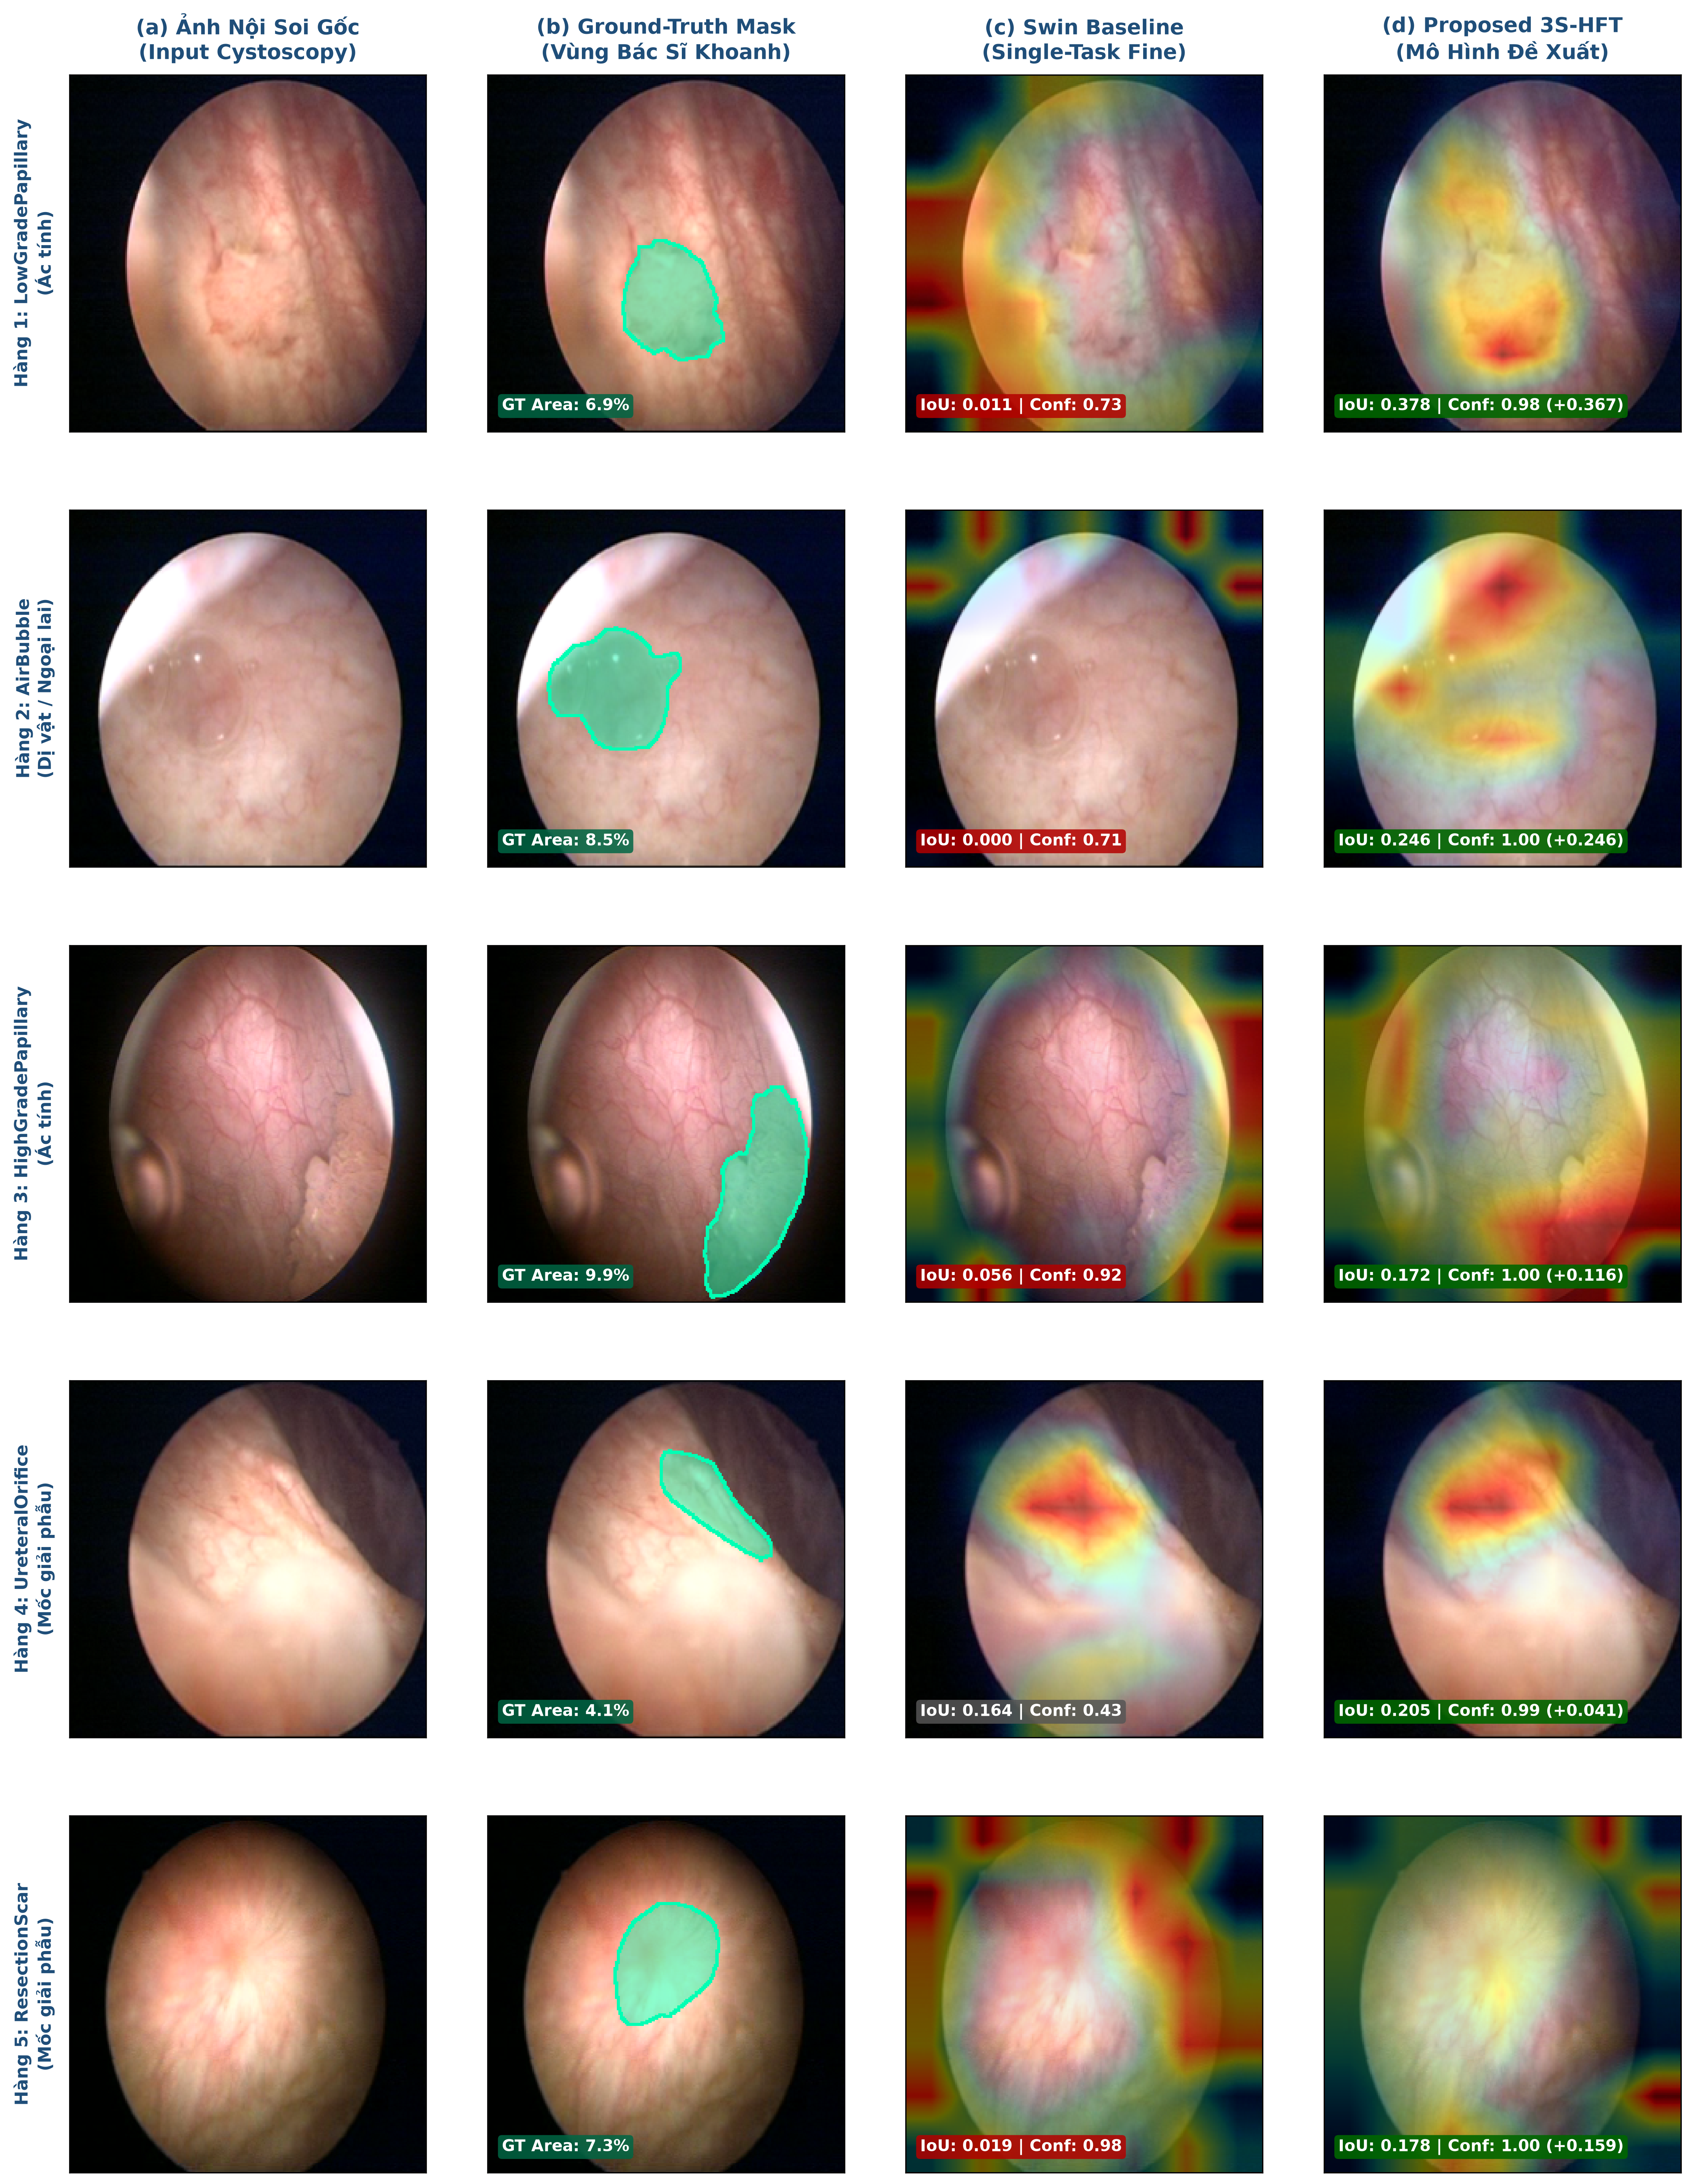
\includegraphics[width=\linewidth,keepaspectratio]{paper_assets/fig_gradcam_comparison.png}
\caption{So sánh đối chuẩn bản đồ nhiệt Grad-CAM giữa mô hình Swin Baseline và CystoHier trên 5 phân lớp chẩn đoán có mặt nạ Ground-Truth. (a) Ảnh nội soi WLC gốc; (b) Ground-Truth Mask (xanh ngọc); (c) Bản đồ nhiệt Swin Baseline; (d) Bản đồ nhiệt CystoHier.}
\label{fig:fig3}
\end{figure}


\begin{table}[htbp]
\centering
\caption{Bảng 11.}
\label{tab:table11}
\vspace{2pt}
\resizebox{\linewidth}{!}{
\begin{tabular}{lrrrrrrr}
\toprule
\# & Phân Lớp Chẩn Đoán & Nhóm Coarse & Nguồn Mẫu & Swin IoU (\%) & CystoHier Conf. & CystoHier IoU (\%) & Mức Nâng Cao (\(\Delta\)) \\
\midrule
1 & \textbf{Low\allowbreak{}Grade\allowbreak{}Papillary} & Ác tính & Test Hold-out & 1.12\% &
0.979 & \textbf{37.78\%} & \textbf{+36.66 pp} \\
2 & \textbf{AirBubble} & Dị vật & Test Hold-out & 0.00\% & 1.000 &
\textbf{24.60\%} & \textbf{+24.60 pp} \\
3 & \textbf{High\allowbreak{}Grade\allowbreak{}Papillary} & Ác tính & Test Hold-out & 5.56\% &
1.000 & \textbf{17.17\%} & \textbf{+11.61 pp} \\
4 & \textbf{UreteralOrifice} & Mốc giải phẫu & Test Hold-out & 16.44\% &
0.993 & \textbf{20.50\%} & \textbf{+4.06 pp} \\
5 & \textbf{ResectionScar} & Mốc giải phẫu & Test Hold-out & 1.87\% &
1.000 & \textbf{17.77\%} & \textbf{+15.90 pp} \\
\textbf{TB} & \textbf{Trung Bình Toàn Bộ} & --- & --- & \textbf{5.00\%}
& \textbf{0.994} & \textbf{23.56\%} & \textbf{+18.56 pp (4.71× rel.)} \\
\bottomrule
\end{tabular}
}
\end{table}

\begin{itemize}
\tightlist
\item
  \textbf{Phân tích định lượng Grad-CAM:} Đánh giá định lượng Grad-CAM
  IoU với ngưỡng cố định \(T=0{,}5\) cho thấy mô hình \textbf{CystoHier}
  đạt IoU trung bình \textbf{23,56\% \(\pm\) 7,3\%} so với Swin Baseline
  (\textbf{5,00\%}), tương ứng mức tăng \(+18{,}56\) percentage points
  (pp). Đặc biệt trên phân lớp tổn thương ác tính
  \emph{Low\allowbreak{}Grade\allowbreak{}Papillary}, IoU tăng từ \(1{,}12\%\) lên
  \textbf{37,78\%} (\(+36{,}66\) pp). Mô hình đề xuất giảm thiểu kích
  hoạt giả tại viền đen camera và vùng lóa sáng, cho thấy sự tập trung
  cao hơn vào các vùng có mức độ tương đồng lớn hơn với Ground-Truth
  mask.
\item
  \textbf{Phân tích Độ Nhạy Ngưỡng (Threshold Sensitivity):}

  \begin{itemize}
  \tightlist
  \item
    \(T=0{,}3\): Baseline IoU = \(5{,}71\%\) (Dice = 0,108) \(\to\)
    CystoHier IoU = \(\mathbf{14{,}89\%}\) (Dice = 0,259, tăng
    \(2{,}61\times\)).
  \item
    \(T=0{,}4\): Baseline IoU = \(5{,}26\%\) (Dice = 0,100) \(\to\)
    CystoHier IoU = \(\mathbf{17{,}85\%}\) (Dice = 0,303, tăng
    \(3{,}39\times\)).
  \item
    \(T=0{,}5\): Baseline IoU = \(5{,}00\%\) (Dice = 0,095) \(\to\)
    CystoHier IoU = \(\mathbf{23{,}56\%}\) (Dice = 0,381, tăng
    \(4{,}71\times\)).
  \item
    \(T=0{,}6\): Baseline IoU = \(4{,}55\%\) (Dice = 0,087) \(\to\)
    CystoHier IoU = \(\mathbf{22{,}47\%}\) (Dice = 0,367, tăng
    \(4{,}94\times\)).
  \end{itemize}
\end{itemize}

\subsection{6.2. Hiệu năng suy luận thực tế trên thiết bị
biên}\label{hiux1ec7u-nux103ng-suy-luux1eadn-thux1ef1c-tux1ebf-truxean-thiux1ebft-bux1ecb-biuxean}

\begin{table}[htbp]
\centering
\caption{Bảng 12.}
\label{tab:table12}
\vspace{2pt}
\resizebox{\linewidth}{!}{
\begin{tabular}{lllllll}
\toprule
Chế Độ / Batch & Số Vòng Đo & Forward Model (ms/ảnh) & Thông Lượng Forward (FPS) & Pipeline End-to-End (ms) & Thông Lượng End-to-End (FPS) & Bộ Nhớ MPS \\
\midrule
\textbf{Batch = 1 (Đơn ảnh)} & 60 & \textbf{12.081 ± 0.95 ms} &
\textbf{82.78 FPS} & \textbf{15.000 ± 1.12 ms} & \textbf{66.67 FPS} &
110.83 MiB \\
\textbf{Batch = 8 (Mini-batch)} & 60 & \textbf{10.167 ± 0.42 ms} &
\textbf{98.36 FPS} & --- & --- & 113.99 MiB \\
\textbf{Batch = 32 (Thông lượng cao)} & 20 & \textbf{9.954 ± 0.38 ms} &
\textbf{100.46 FPS} & --- & --- & 128.00 MiB \\
\bottomrule
\end{tabular}
}
\end{table}

\begin{itemize}
\tightlist
\item
  \textbf{Tính khả thi lâm sàng:} Thông lượng suy luận toàn trình đo
  được là \textbf{66,67 FPS} (độ trễ 15,00 ms/ảnh), cho thấy mô hình có
  đủ thông lượng tính toán cho xử lý khung hình thời gian thực trong
  pipeline suy luận được đánh giá.
\end{itemize}

\subsection{6.3. Giới hạn nghiên cứu \& Hướng phát
triển}\label{giux1edbi-hux1ea1n-nghiuxean-cux1ee9u-hux1b0ux1edbng-phuxe1t-triux1ec3n}

\begin{enumerate}
\def\labelenumi{\arabic{enumi}.}
\tightlist
\item
  \textbf{Thiên lệch chẩn đoán an toàn:} Các trường hợp chẩn đoán sai
  lệch giữa nhóm \emph{Non-malignant} và \emph{Malignant} (26/32 ảnh)
  chủ yếu do mô hình có xu hướng cảnh báo an toàn (\emph{overcalling})
  nhằm tránh bỏ sót tổn thương tiền ung thư. Xu hướng dự đoán thận trọng
  này có thể hữu ích trong tầm soát; tuy nhiên, giá trị lâm sàng thực tế
  cần được kiểm chứng trong các nghiên cứu tiền cứu.
\item
  \textbf{Cỡ mẫu ngoại kiểm hồi cứu:} Nghiên cứu hiện tại kiểm định trên
  23 bệnh nhân của tập Lazo et al.~Các nghiên cứu tiếp theo cần mở rộng
  sang thử nghiệm tiền cứu đa trung tâm và tích hợp mạng Temporal Video
  Transformer cho chuỗi video liên tục.
\end{enumerate}

\begin{center}\rule{0.5\linewidth}{0.5pt}\end{center}

\section{7. Kết luận (Conclusion)}\label{kux1ebft-luux1eadn-conclusion}

CystoHier consistently improved fine-grained classification and
hierarchical consistency over the evaluated baselines under
patient-disjoint validation, while maintaining strong binary
discrimination. Zero-shot evaluation on the independent Lazo cohort
further demonstrated robust cross-dataset generalization, including
under NBI imaging. The model also achieved real-time inference
throughput on Apple Silicon. These results support the feasibility of
hierarchical long-tailed learning for cystoscopic image analysis, while
prospective multicenter validation remains necessary before clinical
deployment.

{[}1{]} Lee TJ, Qiu L, Long J, \emph{et al.} CystoDS: a multiclass
endoscopy image dataset for artificial intelligence-assisted bladder
cancer detection. \emph{Scientific Data}. 2026. doi:
\href{https://doi.org/10.1038/s41597-026-06887-z}{10.1038/s41597-026-06887-z}.

{[}2{]} Liu Z, Lin Y, Cao Y, \emph{et al.} Swin Transformer:
Hierarchical Vision Transformer using Shifted Windows. \emph{Proceedings
of ICCV}. 2021. doi:
\href{https://doi.org/10.1109/ICCV48922.2021.00986}{10.1109/ICCV48922.2021.00986}.

{[}3{]} Ren J, Yu C, Ma X, Zhao H, Yi S. Balanced Meta-Softmax for
Long-Tailed Visual Recognition. \emph{NeurIPS}. 2020.

{[}4{]} Khosla P, Teterwak P, Wang C, \emph{et al.} Supervised
Contrastive Learning. \emph{NeurIPS}. 2020.

{[}5{]} Shkolyar E, Jia X, Chang TC, \emph{et al.} Augmented Bladder
Tumor Detection Using Deep Learning. \emph{European Urology}.
2019;76(6):714--718. doi:
\href{https://doi.org/10.1016/j.eururo.2019.08.032}{10.1016/j.eururo.2019.08.032}.

{[}6{]} Wu S, Chen X, Pan J, \emph{et al.} An Artificial Intelligence
System for the Detection of Bladder Cancer via Cystoscopy: A Multicenter
Diagnostic Study. \emph{Journal of the National Cancer Institute}.
2022;114(2):220--227. doi:
\href{https://doi.org/10.1093/jnci/djab179}{10.1093/jnci/djab179}.

{[}7{]} Lazo Sanchez J, Rosa B, Cattellani M, \emph{et al.}
Semi-supervised Bladder Tissue Classification in Multi-Domain Endoscopic
Images. \emph{IEEE Transactions on Biomedical Engineering}.
2023;70(10):2822--2833. doi:
\href{https://doi.org/10.1109/TBME.2023.3265679}{10.1109/TBME.2023.3265679}.

{[}8{]} Jia X, Shkolyar E, Laurie MA, \emph{et al.} Tumor detection
under cystoscopy with transformer-augmented deep learning algorithm.
\emph{Physics in Medicine \& Biology}. 2023;68(16):165013. doi:
\href{https://doi.org/10.1088/1361-6560/ace499}{10.1088/1361-6560/ace499}.

{[}9{]} Abd El-Aziz AA, Mahmood MA, Abd El-Ghany S.
EfficientNet-B3-Based Automated Deep Learning Framework for Multiclass
Endoscopic Bladder Tissue Classification. \emph{Diagnostics}.
2025;15(19):2515. doi:
\href{https://doi.org/10.3390/diagnostics15192515}{10.3390/diagnostics15192515}.

{[}10{]} Wang Y, Liang H, Zhang Y, \emph{et al.} Artificial intelligence
diagnostics for bladder tumor identification and grade prediction depend
on narrow band imaging cystoscopy. \emph{iScience}. 2026;29(2):114309.
doi:
\href{https://doi.org/10.1016/j.isci.2025.114309}{10.1016/j.isci.2025.114309}.

{[}11{]} Zhang F, An J, Zhao L, \emph{et al.} Artificial
Intelligence-Powered Cystoscopy Diagnostic Support System: Clinical
Application of Multiarchitecture Deep Learning Models. \emph{Journal of
Endourology}. 2026;40(8):925--934. doi:
\href{https://doi.org/10.1177/08927790261450807}{10.1177/08927790261450807}.

{[}12{]} He K, Zhang X, Ren S, Sun J. Deep Residual Learning for Image
Recognition. \emph{Proceedings of CVPR}. 2016. doi:
\href{https://doi.org/10.1109/CVPR.2016.90}{10.1109/CVPR.2016.90}.

{[}13{]} Xie S, Girshick R, Dollár P, Tu Z, He K. Aggregated Residual
Transformations for Deep Neural Networks. \emph{Proceedings of CVPR}.
2017. doi:
\href{https://doi.org/10.1109/CVPR.2017.634}{10.1109/CVPR.2017.634}.

{[}14{]} Sun K, Xiao B, Liu D, Wang J. Deep High-Resolution
Representation Learning for Human Pose Estimation. \emph{Proceedings of
CVPR}. 2019. doi:
\href{https://doi.org/10.1109/CVPR.2019.00584}{10.1109/CVPR.2019.00584}.

{[}15{]} Tan M, Le QV. EfficientNet: Rethinking Model Scaling for
Convolutional Neural Networks. \emph{Proceedings of ICML}. 2019.

{[}16{]} Liu Z, Mao H, Wu CY, Feichtenhofer C, Darrell T, Xie S. A
ConvNet for the 2020s. \emph{Proceedings of CVPR}. 2022. doi:
\href{https://doi.org/10.1109/CVPR52688.2022.01167}{10.1109/CVPR52688.2022.01167}.

\end{document}
